% Options for packages loaded elsewhere
\PassOptionsToPackage{unicode}{hyperref}
\PassOptionsToPackage{hyphens}{url}
%
\documentclass[
]{article}
\usepackage{amsmath,amssymb}
\usepackage{iftex}
\ifPDFTeX
  \usepackage[T1]{fontenc}
  \usepackage[utf8]{inputenc}
  \usepackage{textcomp} % provide euro and other symbols
\else % if luatex or xetex
  \usepackage{unicode-math} % this also loads fontspec
  \defaultfontfeatures{Scale=MatchLowercase}
  \defaultfontfeatures[\rmfamily]{Ligatures=TeX,Scale=1}
\fi
\usepackage{lmodern}
\ifPDFTeX\else
  % xetex/luatex font selection
\fi
% Use upquote if available, for straight quotes in verbatim environments
\IfFileExists{upquote.sty}{\usepackage{upquote}}{}
\IfFileExists{microtype.sty}{% use microtype if available
  \usepackage[]{microtype}
  \UseMicrotypeSet[protrusion]{basicmath} % disable protrusion for tt fonts
}{}
\makeatletter
\@ifundefined{KOMAClassName}{% if non-KOMA class
  \IfFileExists{parskip.sty}{%
    \usepackage{parskip}
  }{% else
    \setlength{\parindent}{0pt}
    \setlength{\parskip}{6pt plus 2pt minus 1pt}}
}{% if KOMA class
  \KOMAoptions{parskip=half}}
\makeatother
\usepackage{xcolor}
\usepackage[margin=1in]{geometry}
\usepackage{color}
\usepackage{fancyvrb}
\newcommand{\VerbBar}{|}
\newcommand{\VERB}{\Verb[commandchars=\\\{\}]}
\DefineVerbatimEnvironment{Highlighting}{Verbatim}{commandchars=\\\{\}}
% Add ',fontsize=\small' for more characters per line
\usepackage{framed}
\definecolor{shadecolor}{RGB}{248,248,248}
\newenvironment{Shaded}{\begin{snugshade}}{\end{snugshade}}
\newcommand{\AlertTok}[1]{\textcolor[rgb]{0.94,0.16,0.16}{#1}}
\newcommand{\AnnotationTok}[1]{\textcolor[rgb]{0.56,0.35,0.01}{\textbf{\textit{#1}}}}
\newcommand{\AttributeTok}[1]{\textcolor[rgb]{0.13,0.29,0.53}{#1}}
\newcommand{\BaseNTok}[1]{\textcolor[rgb]{0.00,0.00,0.81}{#1}}
\newcommand{\BuiltInTok}[1]{#1}
\newcommand{\CharTok}[1]{\textcolor[rgb]{0.31,0.60,0.02}{#1}}
\newcommand{\CommentTok}[1]{\textcolor[rgb]{0.56,0.35,0.01}{\textit{#1}}}
\newcommand{\CommentVarTok}[1]{\textcolor[rgb]{0.56,0.35,0.01}{\textbf{\textit{#1}}}}
\newcommand{\ConstantTok}[1]{\textcolor[rgb]{0.56,0.35,0.01}{#1}}
\newcommand{\ControlFlowTok}[1]{\textcolor[rgb]{0.13,0.29,0.53}{\textbf{#1}}}
\newcommand{\DataTypeTok}[1]{\textcolor[rgb]{0.13,0.29,0.53}{#1}}
\newcommand{\DecValTok}[1]{\textcolor[rgb]{0.00,0.00,0.81}{#1}}
\newcommand{\DocumentationTok}[1]{\textcolor[rgb]{0.56,0.35,0.01}{\textbf{\textit{#1}}}}
\newcommand{\ErrorTok}[1]{\textcolor[rgb]{0.64,0.00,0.00}{\textbf{#1}}}
\newcommand{\ExtensionTok}[1]{#1}
\newcommand{\FloatTok}[1]{\textcolor[rgb]{0.00,0.00,0.81}{#1}}
\newcommand{\FunctionTok}[1]{\textcolor[rgb]{0.13,0.29,0.53}{\textbf{#1}}}
\newcommand{\ImportTok}[1]{#1}
\newcommand{\InformationTok}[1]{\textcolor[rgb]{0.56,0.35,0.01}{\textbf{\textit{#1}}}}
\newcommand{\KeywordTok}[1]{\textcolor[rgb]{0.13,0.29,0.53}{\textbf{#1}}}
\newcommand{\NormalTok}[1]{#1}
\newcommand{\OperatorTok}[1]{\textcolor[rgb]{0.81,0.36,0.00}{\textbf{#1}}}
\newcommand{\OtherTok}[1]{\textcolor[rgb]{0.56,0.35,0.01}{#1}}
\newcommand{\PreprocessorTok}[1]{\textcolor[rgb]{0.56,0.35,0.01}{\textit{#1}}}
\newcommand{\RegionMarkerTok}[1]{#1}
\newcommand{\SpecialCharTok}[1]{\textcolor[rgb]{0.81,0.36,0.00}{\textbf{#1}}}
\newcommand{\SpecialStringTok}[1]{\textcolor[rgb]{0.31,0.60,0.02}{#1}}
\newcommand{\StringTok}[1]{\textcolor[rgb]{0.31,0.60,0.02}{#1}}
\newcommand{\VariableTok}[1]{\textcolor[rgb]{0.00,0.00,0.00}{#1}}
\newcommand{\VerbatimStringTok}[1]{\textcolor[rgb]{0.31,0.60,0.02}{#1}}
\newcommand{\WarningTok}[1]{\textcolor[rgb]{0.56,0.35,0.01}{\textbf{\textit{#1}}}}
\usepackage{graphicx}
\makeatletter
\def\maxwidth{\ifdim\Gin@nat@width>\linewidth\linewidth\else\Gin@nat@width\fi}
\def\maxheight{\ifdim\Gin@nat@height>\textheight\textheight\else\Gin@nat@height\fi}
\makeatother
% Scale images if necessary, so that they will not overflow the page
% margins by default, and it is still possible to overwrite the defaults
% using explicit options in \includegraphics[width, height, ...]{}
\setkeys{Gin}{width=\maxwidth,height=\maxheight,keepaspectratio}
% Set default figure placement to htbp
\makeatletter
\def\fps@figure{htbp}
\makeatother
\setlength{\emergencystretch}{3em} % prevent overfull lines
\providecommand{\tightlist}{%
  \setlength{\itemsep}{0pt}\setlength{\parskip}{0pt}}
\setcounter{secnumdepth}{-\maxdimen} % remove section numbering
\usepackage{listings}
\lstset{breaklines=true}
\usepackage{booktabs}
\usepackage{longtable}
\usepackage{array}
\usepackage{multirow}
\usepackage{wrapfig}
\usepackage{float}
\usepackage{colortbl}
\usepackage{pdflscape}
\usepackage{tabu}
\usepackage{threeparttable}
\usepackage{threeparttablex}
\usepackage[normalem]{ulem}
\usepackage{makecell}
\usepackage{xcolor}
\ifLuaTeX
  \usepackage{selnolig}  % disable illegal ligatures
\fi
\IfFileExists{bookmark.sty}{\usepackage{bookmark}}{\usepackage{hyperref}}
\IfFileExists{xurl.sty}{\usepackage{xurl}}{} % add URL line breaks if available
\urlstyle{same}
\hypersetup{
  pdftitle={MovieLens Capstone Project},
  pdfauthor={Robert Gravelle},
  hidelinks,
  pdfcreator={LaTeX via pandoc}}

\title{\centering MovieLens Capstone Project}
\usepackage{etoolbox}
\makeatletter
\providecommand{\subtitle}[1]{% add subtitle to \maketitle
  \apptocmd{\@title}{\par {\large #1 \par}}{}{}
}
\makeatother
\subtitle{Professional Certificate PH125.9x}
\author{Robert Gravelle}
\date{2023-11-13}

\begin{document}
\maketitle

{
\setcounter{tocdepth}{2}
\tableofcontents
}
\begin{figure}
\centering
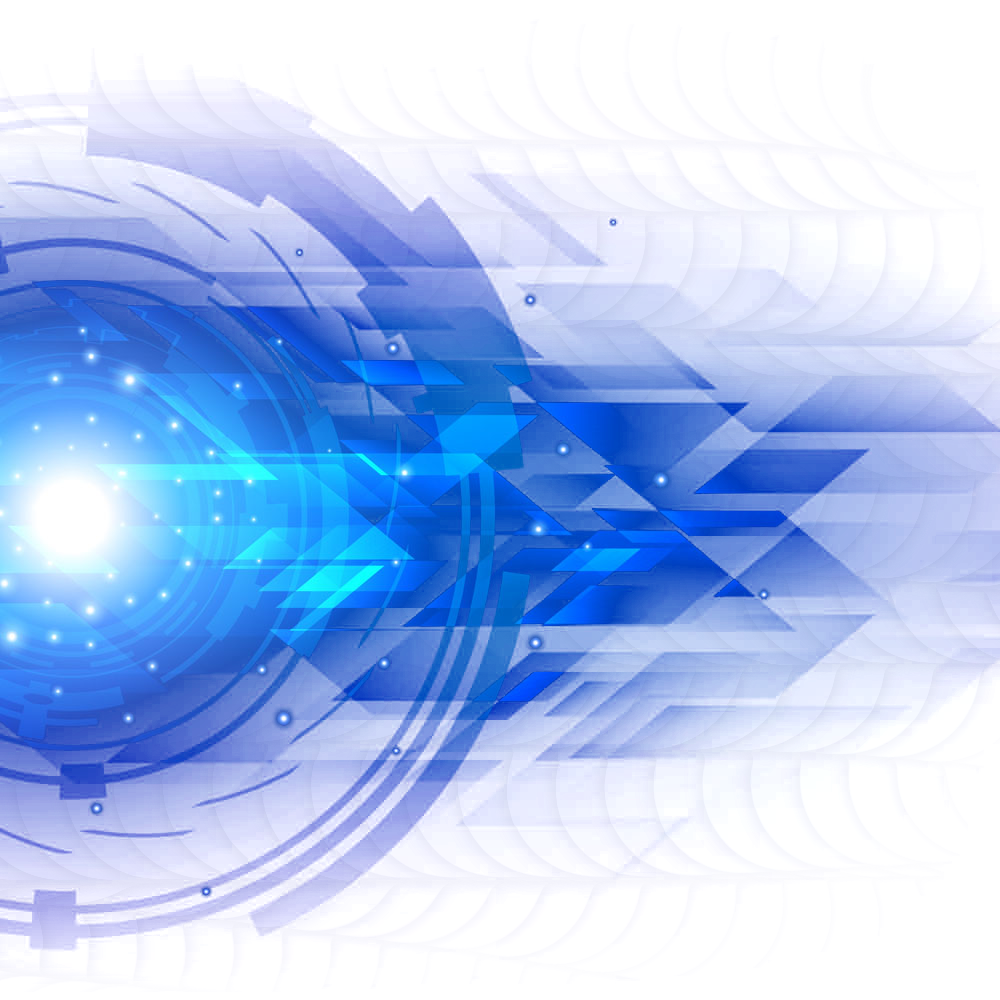
\includegraphics{C:/RProj/MovieLens/MovieLens/graphic.png}
\caption{Background Image}
\end{figure}

\newpage

\hypertarget{movielens}{%
\section{MovieLens}\label{movielens}}

\hypertarget{introduction}{%
\subsection{Introduction}\label{introduction}}

This report delves into the analysis of MovieLens data, encompassing the
training of a recommendation model and assessing its performance.
Initially, we embark on exploring and potentially refining the dataset,
subjecting it to inspection for a comprehensive evaluation of potential
training strategies. Subsequently, the focus shifts to constructing a
machine learning model dedicated to suggesting movies to users.

\hypertarget{dataset-information}{%
\subsection{Dataset Information}\label{dataset-information}}

The 10M MovieLens dataset is a rich repository of cinematic insights,
containing 10 million user-generated ratings across a spectrum of 10,000
movies. This expansive collection captures the diverse perspectives of
72,000 randomly selected users, offering a nuanced glimpse into the
tapestry of audience preferences. This dataset serves as a valuable
foundation for in-depth analyses and the development of robust
recommendation models within the realm of movie suggestions.

\hypertarget{initial-project-configuration}{%
\subsection{Initial Project
Configuration}\label{initial-project-configuration}}

In this project I initiated the loading process of the MovieLens 10M
dataset, meticulously partitioning it into two subsets: \emph{edx} and
\emph{final\_holdout\_test}. These subsets, constituting 10\% of the
entire MovieLens data, serve a specific purpose---solely reserved for
conclusive validation towards the project's conclusion. In preparing
this dataset, key elements used are: userId, movieId, rating, timestamp,
title, and genre. Together, they form the foundational components of
this dynamic dataset, prepared for detailed exploration and validation..

\hypertarget{goal}{%
\subsection{Goal}\label{goal}}

This dataset serves as a portal for exploration, providing valuable
insights into the intricate process of crafting an effective
recommendation algorithm. The quest for a machine learning algorithm led
me to a robust and meticulously developed algorithm to rigorously test
against the dataset of the final\_holdout\_test set. The meticulous
process ensures the algorithm's robustness and efficacy in pursuing an
efficient program of movie recommendations.

\hypertarget{summary}{%
\subsection{Summary}\label{summary}}

The analysis revealed interesting properties and correlations of the
various features. Among other things, older films tended to be rated
higher than newer ones, and some genres were generally rated slightly
higher or lower. Above all, however, the films and the users play a
decisive role in developing a model. Unfortunately, only an RMSE of
about 0.879 was possible with this method. For further interesting model
trainings neither the time nor the available computing power was
sufficient, for example other training approaches like KNN or Decision
Tree could be tried.

\newpage

\hypertarget{code-provided-by-edx-in-the-capstone-directons-for-the-project}{%
\subsection{Code provided by EdX in the Capstone directons for the
project}\label{code-provided-by-edx-in-the-capstone-directons-for-the-project}}

\begin{quote}
\begin{Shaded}
\begin{Highlighting}[]
\CommentTok{\# Create edx and final\_holdout\_test sets}

\CommentTok{\# Note: this process could take a couple of minutes}

\ControlFlowTok{if}\NormalTok{(}\SpecialCharTok{!}\FunctionTok{require}\NormalTok{(tidyverse)) }\FunctionTok{install.packages}\NormalTok{(}\StringTok{"tidyverse"}\NormalTok{, }\AttributeTok{repos =} \StringTok{"http://cran.us.r{-}project.org"}\NormalTok{)}
\ControlFlowTok{if}\NormalTok{(}\SpecialCharTok{!}\FunctionTok{require}\NormalTok{(caret)) }\FunctionTok{install.packages}\NormalTok{(}\StringTok{"caret"}\NormalTok{, }\AttributeTok{repos =} \StringTok{"http.cran.us.r{-}project.org"}\NormalTok{)}

\FunctionTok{library}\NormalTok{(tidyverse)}
\FunctionTok{library}\NormalTok{(caret)}

\CommentTok{\# MovieLens 10M dataset:}
\CommentTok{\# https://grouplens.org/datasets/movielens/10m/}
\CommentTok{\# http://files.grouplens.org/datasets/movielens/ml{-}10m.zip}

\FunctionTok{options}\NormalTok{(}\AttributeTok{timeout =} \DecValTok{250}\NormalTok{)}

\NormalTok{dl }\OtherTok{\textless{}{-}} \StringTok{"ml{-}10M100K.zip"}
\ControlFlowTok{if}\NormalTok{(}\SpecialCharTok{!}\FunctionTok{file.exists}\NormalTok{(dl))}
  \FunctionTok{download.file}\NormalTok{(}\StringTok{"https://files.grouplens.org/datasets/movielens/ml{-}10m.zip"}\NormalTok{, dl)}

\NormalTok{ratings\_file }\OtherTok{\textless{}{-}} \StringTok{"ml{-}10M100K/ratings.dat"}
\ControlFlowTok{if}\NormalTok{(}\SpecialCharTok{!}\FunctionTok{file.exists}\NormalTok{(ratings\_file))}
  \FunctionTok{unzip}\NormalTok{(dl, ratings\_file)}

\NormalTok{movies\_file }\OtherTok{\textless{}{-}} \StringTok{"ml{-}10M100K/movies.dat"}
\ControlFlowTok{if}\NormalTok{(}\SpecialCharTok{!}\FunctionTok{file.exists}\NormalTok{(movies\_file))}
  \FunctionTok{unzip}\NormalTok{(dl, movies\_file)}

\NormalTok{ratings }\OtherTok{\textless{}{-}} \FunctionTok{as.data.frame}\NormalTok{(}\FunctionTok{str\_split}\NormalTok{(}\FunctionTok{read\_lines}\NormalTok{(ratings\_file), }\FunctionTok{fixed}\NormalTok{(}\StringTok{"::"}\NormalTok{), }\AttributeTok{simplify =} \ConstantTok{TRUE}\NormalTok{),}
                         \AttributeTok{stringsAsFactors =} \ConstantTok{FALSE}\NormalTok{)}
\FunctionTok{colnames}\NormalTok{(ratings) }\OtherTok{\textless{}{-}} \FunctionTok{c}\NormalTok{(}\StringTok{"userId"}\NormalTok{, }\StringTok{"movieId"}\NormalTok{, }\StringTok{"rating"}\NormalTok{, }\StringTok{"timestamp"}\NormalTok{)}
\NormalTok{ratings }\OtherTok{\textless{}{-}}\NormalTok{ ratings }\SpecialCharTok{\%\textgreater{}\%}
  \FunctionTok{mutate}\NormalTok{(}\AttributeTok{userId =} \FunctionTok{as.integer}\NormalTok{(userId),}
         \AttributeTok{movieId =} \FunctionTok{as.integer}\NormalTok{(movieId),}
         \AttributeTok{rating =} \FunctionTok{as.numeric}\NormalTok{(rating),}
         \AttributeTok{timestamp =} \FunctionTok{as.integer}\NormalTok{(timestamp))}

\NormalTok{movies }\OtherTok{\textless{}{-}} \FunctionTok{as.data.frame}\NormalTok{(}\FunctionTok{str\_split}\NormalTok{(}\FunctionTok{read\_lines}\NormalTok{(movies\_file), }\FunctionTok{fixed}\NormalTok{(}\StringTok{"::"}\NormalTok{), }\AttributeTok{simplify =} \ConstantTok{TRUE}\NormalTok{),}
                        \AttributeTok{stringsAsFactors =} \ConstantTok{FALSE}\NormalTok{)}
\FunctionTok{colnames}\NormalTok{(movies) }\OtherTok{\textless{}{-}} \FunctionTok{c}\NormalTok{(}\StringTok{"movieId"}\NormalTok{, }\StringTok{"title"}\NormalTok{, }\StringTok{"genres"}\NormalTok{)}
\NormalTok{movies }\OtherTok{\textless{}{-}}\NormalTok{ movies }\SpecialCharTok{\%\textgreater{}\%}
  \FunctionTok{mutate}\NormalTok{(}\AttributeTok{movieId =} \FunctionTok{as.integer}\NormalTok{(movieId))}

\NormalTok{movielens }\OtherTok{\textless{}{-}} \FunctionTok{left\_join}\NormalTok{(ratings, movies, }\AttributeTok{by =} \StringTok{"movieId"}\NormalTok{)}

\CommentTok{\# Final hold{-}out test set will be 10\% of MovieLens data}
\FunctionTok{set.seed}\NormalTok{(}\DecValTok{1}\NormalTok{, }\AttributeTok{sample.kind=}\StringTok{"Rounding"}\NormalTok{) }\CommentTok{\# if using R 3.6 or later}
\end{Highlighting}
\end{Shaded}

\begin{verbatim}
## Warning in set.seed(1, sample.kind = "Rounding"): non-uniform 'Rounding'
## sampler used
\end{verbatim}

\begin{Shaded}
\begin{Highlighting}[]
\CommentTok{\# set.seed(1) \# if using R 3.5 or earlier}
\NormalTok{test\_index }\OtherTok{\textless{}{-}} \FunctionTok{createDataPartition}\NormalTok{(}\AttributeTok{y =}\NormalTok{ movielens}\SpecialCharTok{$}\NormalTok{rating, }\AttributeTok{times =} \DecValTok{1}\NormalTok{, }\AttributeTok{p =} \FloatTok{0.1}\NormalTok{, }\AttributeTok{list =} \ConstantTok{FALSE}\NormalTok{)}
\NormalTok{edx }\OtherTok{\textless{}{-}}\NormalTok{ movielens[}\SpecialCharTok{{-}}\NormalTok{test\_index,]}
\NormalTok{temp }\OtherTok{\textless{}{-}}\NormalTok{ movielens[test\_index,]}

\CommentTok{\# Make sure userId and movieId in final hold{-}out test set are also in edx set}
\NormalTok{final\_holdout\_test }\OtherTok{\textless{}{-}}\NormalTok{ temp }\SpecialCharTok{\%\textgreater{}\%} 
  \FunctionTok{semi\_join}\NormalTok{(edx, }\AttributeTok{by =} \StringTok{"movieId"}\NormalTok{) }\SpecialCharTok{\%\textgreater{}\%}
  \FunctionTok{semi\_join}\NormalTok{(edx, }\AttributeTok{by =} \StringTok{"userId"}\NormalTok{)}

\CommentTok{\# Add rows removed from final hold{-}out test set back into edx set}
\NormalTok{removed }\OtherTok{\textless{}{-}} \FunctionTok{anti\_join}\NormalTok{(temp, final\_holdout\_test)}
\end{Highlighting}
\end{Shaded}

\begin{verbatim}
## Joining with `by = join_by(userId, movieId, rating, timestamp, title, genres)`
\end{verbatim}
\end{quote}

\newpage

\hypertarget{analysis}{%
\section{Analysis}\label{analysis}}

\hypertarget{data-inspection-and-preprocessing}{%
\subsection{Data Inspection and
preprocessing}\label{data-inspection-and-preprocessing}}

Let's begin by examining the structure and contents of the Edx dataset
in closer detail.

\begin{table}[!h]
\centering\begingroup\fontsize{8}{10}\selectfont

\begin{tabular}{l|r|r|r|r|l|l}
\hline
  & userId & movieId & rating & timestamp & title & genres\\
\hline
1 & 1 & 122 & 5 & 838985046 & Boomerang (1992) & Comedy|Romance\\
\hline
2 & 1 & 185 & 5 & 838983525 & Net, The (1995) & Action|Crime|Thriller\\
\hline
4 & 1 & 292 & 5 & 838983421 & Outbreak (1995) & Action|Drama|Sci-Fi|Thriller\\
\hline
5 & 1 & 316 & 5 & 838983392 & Stargate (1994) & Action|Adventure|Sci-Fi\\
\hline
6 & 1 & 329 & 5 & 838983392 & Star Trek: Generations (1994) & Action|Adventure|Drama|Sci-Fi\\
\hline
\end{tabular}
\endgroup{}
\end{table}

This dataset comprises various columns, each providing crucial
information:

\begin{itemize}
\tightlist
\item
  \textbf{userId}: Uniquely identifies the user who rated the movie.
\item
  \textbf{movieId}: Serves as a distinctive identifier for the rated
  movie.
\item
  \textbf{rating}: Indicates the user-assigned rating for the movie,
  with the rating scale yet to be determined.
\item
  \textbf{timestamp}: Presents the timestamp in UNIX format.
\item
  \textbf{title}: Encompasses the movie's title, inclusive of its
  release year.
\item
  \textbf{genres}: Enumerates a set of genres linked to the movie, with
  multiple genres separated by `\textbar{}'.
\end{itemize}

Within the realms of the edx dataset, a multitude of captivating
explorations await:

\begin{enumerate}
\def\labelenumi{\arabic{enumi}.}
\tightlist
\item
  \textbf{Exceptional Cinematic Appeal:}

  \begin{itemize}
  \tightlist
  \item
    Identify movies that soar above the average rating, potentially
    fueled by compelling narratives or impeccable production.
  \end{itemize}
\item
  \textbf{Genre Elevation:}

  \begin{itemize}
  \tightlist
  \item
    Scrutinize variations in ratings across different genres or their
    combinations, unveiling those that consistently receive higher
    acclaim.
  \end{itemize}
\item
  \textbf{User Rating Dynamics:}

  \begin{itemize}
  \tightlist
  \item
    Delve into the potential bias within user ratings, discerning
    whether there's a prevalent inclination towards loftier or lower
    ratings overall.
  \end{itemize}
\item
  \textbf{Genre Affinity Impact:}

  \begin{itemize}
  \tightlist
  \item
    Investigate how individual user genre preferences influence their
    ratings. For instance, a user inclined towards Horror and Action may
    tend to rate movies outside these genres lower.
  \end{itemize}
\item
  \textbf{Temporal Rating Odyssey:}

  \begin{itemize}
  \tightlist
  \item
    Unearth the correlation between user ratings and movie release
    years, potentially revealing evolving patterns or trends over time.
  \end{itemize}
\item
  \textbf{Popularity Quotient:}

  \begin{itemize}
  \tightlist
  \item
    Navigate the landscape of user ratings concerning the popularity
    spectrum, distinguishing between indie and blockbuster films. This
    exploration might unveil distinct rating patterns associated with
    movies of varying popularity levels.
  \end{itemize}
\end{enumerate}

\newpage

Before delving into our analysis, it's imperative to meticulously
inspect the dataset for any missing values or anomalies in unique data
names that might hint at outlier information.

The dataset \emph{edx} contains 0 missing values.

Lets discover the genres in the dataset

\begin{center}


\begin{tabular}{l}
\hline
Genres\\
\hline
Comedy\\
\hline
Romance\\
\hline
Action\\
\hline
Crime\\
\hline
Thriller\\
\hline
Drama\\
\hline
Sci-Fi\\
\hline
Adventure\\
\hline
Children\\
\hline
Fantasy\\
\hline
War\\
\hline
Animation\\
\hline
Musical\\
\hline
Western\\
\hline
Mystery\\
\hline
Film-Noir\\
\hline
Horror\\
\hline
Documentary\\
\hline
IMAX\\
\hline
(no genres listed)\\
\hline
\end{tabular}

 
\end{center}

We notice a unusual genre named in the list of \emph{(no genres
listed)}.

\begin{table}[!h]
\centering\begingroup\fontsize{8}{10}\selectfont

\begin{tabular}{l|r|r|r|r|l|l}
\hline
  & userId & movieId & rating & timestamp & title & genres\\
\hline
1025055 & 7701 & 8606 & 5.0 & 1190806786 & Pull My Daisy (1958) & (no genres listed)\\
\hline
1453345 & 10680 & 8606 & 4.5 & 1171170472 & Pull My Daisy (1958) & (no genres listed)\\
\hline
4066835 & 29097 & 8606 & 2.0 & 1089648625 & Pull My Daisy (1958) & (no genres listed)\\
\hline
6456906 & 46142 & 8606 & 3.5 & 1226518191 & Pull My Daisy (1958) & (no genres listed)\\
\hline
8046611 & 57696 & 8606 & 4.5 & 1230588636 & Pull My Daisy (1958) & (no genres listed)\\
\hline
8988750 & 64411 & 8606 & 3.5 & 1096732843 & Pull My Daisy (1958) & (no genres listed)\\
\hline
9404670 & 67385 & 8606 & 2.5 & 1188277325 & Pull My Daisy (1958) & (no genres listed)\\
\hline
\end{tabular}
\endgroup{}
\end{table}

Upon delving deeper, it came to light that a solitary movie, ``Pull My
Daisy,'' lacks a designated genre. As per IMDB, this 1958 film falls
under the category of ``Short.'' To refine our dataset, let's extract
and categorize the listed genres, allocating the initial three genres of
each movie into distinct columns.

In discovery we see there are 20 unique genres in the EdX dataset.

Next, we convert the UNIX timestamps into a more readable date/time
format and, for convenience, extract the year when the movie was rated.
Additionally, we isolate the release year embedded in the title, laying
the groundwork for potential further exploration.

Now some columns are added for further inspection, lets see the table
again.

\begin{table}[!h]
\centering\begingroup\fontsize{4}{6}\selectfont

\begin{tabular}{l|r|r|r|r|l|l|l|l|l|l|r|r}
\hline
  & userId & movieId & rating & timestamp & title & genres & main\_genre & side1\_genre & side2\_genre & date & yearrated & releaseyear\\
\hline
1 & 1 & 122 & 5 & 838985046 & Boomerang (1992) & Comedy|Romance & Comedy & Romance & NA & 1996-08-02 11:24:06 & 1996 & 1992\\
\hline
2 & 1 & 185 & 5 & 838983525 & Net, The (1995) & Action|Crime|Thriller & Action & Crime & Thriller & 1996-08-02 10:58:45 & 1996 & 1995\\
\hline
4 & 1 & 292 & 5 & 838983421 & Outbreak (1995) & Action|Drama|Sci-Fi|Thriller & Action & Drama & Sci-Fi & 1996-08-02 10:57:01 & 1996 & 1995\\
\hline
5 & 1 & 316 & 5 & 838983392 & Stargate (1994) & Action|Adventure|Sci-Fi & Action & Adventure & Sci-Fi & 1996-08-02 10:56:32 & 1996 & 1994\\
\hline
6 & 1 & 329 & 5 & 838983392 & Star Trek: Generations (1994) & Action|Adventure|Drama|Sci-Fi & Action & Adventure & Drama & 1996-08-02 10:56:32 & 1996 & 1994\\
\hline
7 & 1 & 355 & 5 & 838984474 & Flintstones, The (1994) & Children|Comedy|Fantasy & Children & Comedy & Fantasy & 1996-08-02 11:14:34 & 1996 & 1994\\
\hline
\end{tabular}
\endgroup{}
\end{table}

\newpage

\hypertarget{distributions-and-plots}{%
\subsection{Distributions and Plots}\label{distributions-and-plots}}

\textbackslash begin\}center\} We need to see the distribution of
Ratings \textbackslash end\{center\}

\includegraphics[width=0.7\linewidth]{MovieLens-final-txfr_files/figure-latex/unnamed-chunk-5-1}

The majority of ratings are whole numbers; Additionally, the
distribution of half-point ratings mirrors the pattern and distribution
of the observed ratings in whole-number ratings.

\newpage

\begin{center} Now lets view the the distribution of the genres.\end{center}

\includegraphics[width=0.7\linewidth]{MovieLens-final-txfr_files/figure-latex/unnamed-chunk-6-1}
The prevalent genres predominantly include Action, Comedy, and Drama.
Yet, delving into the realm of sub-genres unveils a more nuanced
distribution. While Drama, Comedy, and Action still claim the top spots,
their positions undergo subtle shifts. Consequently, Drama emerges as a
frequently paired side genre, harmonizing seamlessly with genres such as
Romance, Thriller, and others.

\includegraphics[width=0.7\linewidth]{MovieLens-final-txfr_files/figure-latex/unnamed-chunk-7-1}

\newpage

\hypertarget{genres}{%
\subsection{Genres}\label{genres}}

\begin{center} Lets now see the Genres graphed against the average rating. \end{center}

\includegraphics[width=0.7\linewidth]{MovieLens-final-txfr_files/figure-latex/unnamed-chunk-8-1}
Genre ratings reveal a preference for ``intellectual'' movie genres,
such as Film-Noir, Crime, and Drama, which consistently garner higher
ratings compared to genres associated with entertainment, like Action,
Fantasy, and Horror. This trend holds true when evaluating the average
ratings of genre combinations, specifically those with more than 50,000
ratings.

\includegraphics[width=0.7\linewidth]{MovieLens-final-txfr_files/figure-latex/unnamed-chunk-9-1}

When taken genre combinations into account, a similar picture is
painted, but some entertainment genre combinations, notably a Action
combination, make it higher up the list
(e.g.~Action\textbar Drama\textbar War, Action\textbar Adventure)

\newpage
\begin{center} Rating distribution of movies \end{center}

\includegraphics[width=0.7\linewidth]{MovieLens-final-txfr_files/figure-latex/unnamed-chunk-10-1}
Only a scant number of movies achieve an average rating surpassing
approximately 4.2. The majority of films fall within the range of 2 and
4.5 in terms of average ratings.

\begin{center} Average rating distribution of users \end{center}

\includegraphics[width=0.7\linewidth]{MovieLens-final-txfr_files/figure-latex/unnamed-chunk-11-1}
\newpage

\hypertarget{user-ratings}{%
\subsection{User Ratings}\label{user-ratings}}

The majority of users tend to rate movies within the range of 3.5 to
4.2, surpassing the average ratings observed in the overall movie rating
distribution.

\begin{center} Number of ratings per user \end{center}

\includegraphics[width=0.7\linewidth]{MovieLens-final-txfr_files/figure-latex/unnamed-chunk-12-1}

\newpage

\hypertarget{trendline-graphs-for-ratingsand-release-dates}{%
\subsection{Trendline Graphs for Ratingsand Release
Dates}\label{trendline-graphs-for-ratingsand-release-dates}}

\begin{center} Trend lines average rating per release year \end{center}

\includegraphics{MovieLens-final-txfr_files/figure-latex/unnamed-chunk-13-1.pdf}
Films from the pre-1970 era tend to receive higher ratings compared to
those released in the last two decades. This phenomenon is a well-known
effect, where only the exceptional works withstand the test of time.

\newpage

\begin{center} Number of released movies per year \end{center}

\includegraphics{MovieLens-final-txfr_files/figure-latex/unnamed-chunk-14-1.pdf}

Movie releases maintained a relatively stable pattern before 1970,
experienced a significant uptick around 1990, and almost reached an
explosive surge in the subsequent years. This surge can likely be
attributed to advancements in technology, production, and market
dynamics, including factors such as the proliferation of movie theaters,
the rise of movie rentals, and television. However, since the late
1990s, the number of movie releases witnessed a sharp decline, reversing
the rapid expansion observed a decade earlier.

\newpage

Ratings distribution over the years, focusing on the period from 1996 to
2008, with data outside this range registered as zero.

\includegraphics{MovieLens-final-txfr_files/figure-latex/unnamed-chunk-15-1.pdf}
\newpage

\begin{center} Movie ratings per year are stable with some outlier \end{center}

Get the average rating of movie per genre but in 5 year bins.

\begin{verbatim}
## `summarise()` has grouped output by 'main_genre'. You can override using the
## `.groups` argument.
\end{verbatim}

\includegraphics{MovieLens-final-txfr_files/figure-latex/unnamed-chunk-16-1.pdf}

Certain genres maintain a steady average rating throughout the years,
while others, such as Horror or Fantasy, exhibit more significant
fluctuations.

\newpage

\hypertarget{modeling}{%
\section{Modeling}\label{modeling}}

Prepare the training and test datasets, and set up a table to track RMSE
results as we refine the model. Based on insights from the mean+movie
approach, it's essential to ensure that the training dataset encompasses
all movieIds. This precaution guards against encountering movieIds in
the test set without corresponding training data. I anticipate a similar
consideration might apply to userId and the primary genre.

\hypertarget{blind-guessing}{%
\subsection{Blind Guessing}\label{blind-guessing}}

Try blind guessing a rating from 0 to 5.

\begin{Shaded}
\begin{Highlighting}[]
\CommentTok{\# Blind guessing}
\NormalTok{guess\_model }\OtherTok{\textless{}{-}} \FunctionTok{sample}\NormalTok{(}\FunctionTok{c}\NormalTok{(}\DecValTok{0}\NormalTok{, }\FloatTok{0.5}\NormalTok{, }\DecValTok{1}\NormalTok{, }\FloatTok{1.5}\NormalTok{, }\DecValTok{2}\NormalTok{, }\FloatTok{2.5}\NormalTok{, }\DecValTok{3}\NormalTok{, }\FloatTok{3.5}\NormalTok{, }\DecValTok{4}\NormalTok{, }\FloatTok{4.5}\NormalTok{, }\DecValTok{5}\NormalTok{), }\FunctionTok{length}\NormalTok{(test\_set}\SpecialCharTok{$}\NormalTok{rating), }\AttributeTok{replace=}\ConstantTok{TRUE}\NormalTok{)}
\end{Highlighting}
\end{Shaded}

The resulting 2.1568093 is still far of the \textless{} 0.8649, no
suprise.

\begin{tabular}{l|r}
\hline
Model & RMSE\\
\hline
Guessing & 2.156809\\
\hline
\end{tabular}

\hypertarget{mean}{%
\subsection{Mean}\label{mean}}

Get the average of all ratings on the training set and use this to
predict a movie.

\begin{Shaded}
\begin{Highlighting}[]
\CommentTok{\# The mean rating for each movie in the training set.}
\NormalTok{avg\_model }\OtherTok{\textless{}{-}} \FunctionTok{mean}\NormalTok{(train\_set}\SpecialCharTok{$}\NormalTok{rating)}
\end{Highlighting}
\end{Shaded}

The average of every movie used for predicting a rating results in
1.0607163. Closer but still far off.

\begin{tabular}{l|r}
\hline
Model & RMSE\\
\hline
Guessing & 2.156809\\
\hline
Avg Model & 1.060716\\
\hline
\end{tabular}

\hypertarget{genre-bias-deviation}{%
\subsection{Genre bias Deviation}\label{genre-bias-deviation}}

Evaluate the genre bias, the deviation from the movie average for each
genre.

\begin{Shaded}
\begin{Highlighting}[]
\CommentTok{\# movie average}
\NormalTok{movie\_avg }\OtherTok{\textless{}{-}} \FunctionTok{mean}\NormalTok{(train\_set}\SpecialCharTok{$}\NormalTok{rating)}
\NormalTok{genre\_bias }\OtherTok{\textless{}{-}}\NormalTok{ train\_set }\SpecialCharTok{\%\textgreater{}\%}
  \FunctionTok{group\_by}\NormalTok{(main\_genre) }\SpecialCharTok{\%\textgreater{}\%}
  \FunctionTok{summarise}\NormalTok{(}\AttributeTok{deviation\_genre =} \FunctionTok{mean}\NormalTok{(rating }\SpecialCharTok{{-}}\NormalTok{ movie\_avg))}

\CommentTok{\# combine genre bias with the test\_set}
\NormalTok{mean\_genre\_model }\OtherTok{\textless{}{-}}\NormalTok{ test\_set }\SpecialCharTok{\%\textgreater{}\%}
  \FunctionTok{inner\_join}\NormalTok{(genre\_bias, }\AttributeTok{by=}\StringTok{"main\_genre"}\NormalTok{)}
\end{Highlighting}
\end{Shaded}

The RMSE is slightly improved at r \{ rmse\_mean\_genre\_model \}
compared to simply taking the average as done previously.

\begin{tabular}{l|r}
\hline
Model & RMSE\\
\hline
Guessing & 2.156809\\
\hline
Avg Model & 1.060716\\
\hline
Genre Model & 1.049044\\
\hline
\end{tabular}

\newpage

\hypertarget{movie-bias-rating}{%
\subsection{Movie bias rating}\label{movie-bias-rating}}

The movie bias represents the variance between the average movie rating
and the overall mean rating.

\begin{Shaded}
\begin{Highlighting}[]
\NormalTok{movie\_bias }\OtherTok{\textless{}{-}}\NormalTok{ train\_set }\SpecialCharTok{\%\textgreater{}\%}
  \FunctionTok{group\_by}\NormalTok{(movieId) }\SpecialCharTok{\%\textgreater{}\%}
  \FunctionTok{summarise}\NormalTok{(}\AttributeTok{deviation\_movie =} \FunctionTok{mean}\NormalTok{(rating }\SpecialCharTok{{-}}\NormalTok{ movie\_avg))}

\NormalTok{mean\_movie\_model }\OtherTok{\textless{}{-}}\NormalTok{ test\_set }\SpecialCharTok{\%\textgreater{}\%}
  \FunctionTok{inner\_join}\NormalTok{(movie\_bias, }\AttributeTok{by=}\StringTok{"movieId"}\NormalTok{)}
\end{Highlighting}
\end{Shaded}

With and RMSE of 0.9438696 we are now in the sub 1 category.

\begin{tabular}{l|r}
\hline
Model & RMSE\\
\hline
Guessing & 2.1568093\\
\hline
Avg Model & 1.0607163\\
\hline
Genre Model & 1.0490436\\
\hline
Movie Model & 0.9438696\\
\hline
\end{tabular}

\hypertarget{user-bias}{%
\subsection{User bias}\label{user-bias}}

Lets inspect the user bias.

\begin{Shaded}
\begin{Highlighting}[]
\NormalTok{user\_bias }\OtherTok{\textless{}{-}}\NormalTok{ train\_set }\SpecialCharTok{\%\textgreater{}\%}
  \FunctionTok{group\_by}\NormalTok{(userId) }\SpecialCharTok{\%\textgreater{}\%}
  \FunctionTok{summarise}\NormalTok{(}\AttributeTok{deviation\_user =} \FunctionTok{mean}\NormalTok{(rating }\SpecialCharTok{{-}}\NormalTok{ movie\_avg))}

\NormalTok{mean\_user\_model }\OtherTok{\textless{}{-}}\NormalTok{ test\_set }\SpecialCharTok{\%\textgreater{}\%}
  \FunctionTok{inner\_join}\NormalTok{(user\_bias, }\AttributeTok{by=}\StringTok{"userId"}\NormalTok{)}
\end{Highlighting}
\end{Shaded}

The user bias results in an RMSE of 0.9795706.

\begin{tabular}{l|r}
\hline
Model & RMSE\\
\hline
Guessing & 2.1568093\\
\hline
Avg Model & 1.0607163\\
\hline
Genre Model & 1.0490436\\
\hline
Movie Model & 0.9438696\\
\hline
User Model & 0.9795706\\
\hline
\end{tabular}

\hypertarget{release-year-bias}{%
\subsection{Release year bias}\label{release-year-bias}}

Lets see if the release year will bring the RMSE down.

\begin{Shaded}
\begin{Highlighting}[]
\NormalTok{releaseyear\_bias }\OtherTok{\textless{}{-}}\NormalTok{ train\_set }\SpecialCharTok{\%\textgreater{}\%}
  \FunctionTok{group\_by}\NormalTok{(releaseyear) }\SpecialCharTok{\%\textgreater{}\%}
  \FunctionTok{summarise}\NormalTok{(}\AttributeTok{deviation\_releaseyear =} \FunctionTok{mean}\NormalTok{(rating }\SpecialCharTok{{-}}\NormalTok{ movie\_avg))}

\NormalTok{mean\_releaseyear\_model }\OtherTok{\textless{}{-}}\NormalTok{ test\_set }\SpecialCharTok{\%\textgreater{}\%}
  \FunctionTok{inner\_join}\NormalTok{(releaseyear\_bias, }\AttributeTok{by=}\StringTok{"releaseyear"}\NormalTok{)}
\end{Highlighting}
\end{Shaded}

The release year of a movie bias results in an RMSE of 1.0496303.

\begin{tabular}{l|r}
\hline
Model & RMSE\\
\hline
Guessing & 2.1568093\\
\hline
Avg Model & 1.0607163\\
\hline
Genre Model & 1.0490436\\
\hline
Movie Model & 0.9438696\\
\hline
User Model & 0.9795706\\
\hline
Release Year Model & 1.0496303\\
\hline
\end{tabular}

\hypertarget{user-and-movie-bias}{%
\subsection{User and Movie bias}\label{user-and-movie-bias}}

Let's add the average rating of a user into the mix.

\begin{Shaded}
\begin{Highlighting}[]
\CommentTok{\# user\_bias is the differnece of the avg user rating to the mean rating}
\NormalTok{user\_bias }\OtherTok{\textless{}{-}}\NormalTok{ train\_set }\SpecialCharTok{\%\textgreater{}\%}
  \FunctionTok{group\_by}\NormalTok{(userId) }\SpecialCharTok{\%\textgreater{}\%}
  \FunctionTok{summarise}\NormalTok{(}\AttributeTok{deviation\_user =} \FunctionTok{mean}\NormalTok{(rating }\SpecialCharTok{{-}}\NormalTok{ movie\_avg))}

\NormalTok{mean\_movie\_user\_model }\OtherTok{\textless{}{-}}\NormalTok{ test\_set }\SpecialCharTok{\%\textgreater{}\%}
  \FunctionTok{inner\_join}\NormalTok{(movie\_bias, }\AttributeTok{by=}\StringTok{"movieId"}\NormalTok{) }\SpecialCharTok{\%\textgreater{}\%}
  \FunctionTok{inner\_join}\NormalTok{(user\_bias, }\AttributeTok{by=}\StringTok{"userId"}\NormalTok{)}
\end{Highlighting}
\end{Shaded}

The user and movie gets us below 0.9. But 0.8867528 is still not near
the desired \textless{} 0.865.

\begin{tabular}{l|r}
\hline
Model & RMSE\\
\hline
Guessing & 2.1568093\\
\hline
Avg Model & 1.0607163\\
\hline
Genre Model & 1.0490436\\
\hline
Movie Model & 0.9438696\\
\hline
User Model & 0.9795706\\
\hline
Release Year Model & 1.0496303\\
\hline
Movie + User Model & 0.8867528\\
\hline
\end{tabular}

\hypertarget{user-and-movie-and-release-year-bias}{%
\subsection{User and Movie and Release Year
bias}\label{user-and-movie-and-release-year-bias}}

To the previous model we add the release year.

\begin{Shaded}
\begin{Highlighting}[]
\NormalTok{mean\_movie\_user\_releaseyear\_model }\OtherTok{\textless{}{-}}\NormalTok{ test\_set }\SpecialCharTok{\%\textgreater{}\%}
  \FunctionTok{left\_join}\NormalTok{(movie\_bias, }\AttributeTok{by=}\StringTok{\textquotesingle{}movieId\textquotesingle{}}\NormalTok{) }\SpecialCharTok{\%\textgreater{}\%}
  \FunctionTok{left\_join}\NormalTok{(user\_bias, }\AttributeTok{by=}\StringTok{\textquotesingle{}userId\textquotesingle{}}\NormalTok{) }\SpecialCharTok{\%\textgreater{}\%}
  \FunctionTok{left\_join}\NormalTok{(releaseyear\_bias, }\AttributeTok{by=}\StringTok{\textquotesingle{}releaseyear\textquotesingle{}}\NormalTok{)}
\end{Highlighting}
\end{Shaded}

With the release year added to the user and movie bias we get 0.9030035.

\begin{tabular}{l|r}
\hline
Model & RMSE\\
\hline
Guessing & 2.1568093\\
\hline
Avg Model & 1.0607163\\
\hline
Genre Model & 1.0490436\\
\hline
Movie Model & 0.9438696\\
\hline
User Model & 0.9795706\\
\hline
Release Year Model & 1.0496303\\
\hline
Movie + User Model & 0.8867528\\
\hline
Movie + User + Release Year Model & 0.9030035\\
\hline
\end{tabular}

\hypertarget{user-movie-and-genre-bias}{%
\subsection{User, Movie and Genre
bias}\label{user-movie-and-genre-bias}}

Now combine user, movie and genre together in a single model.

\begin{Shaded}
\begin{Highlighting}[]
\NormalTok{mean\_movie\_user\_genre\_model }\OtherTok{\textless{}{-}}\NormalTok{ test\_set }\SpecialCharTok{\%\textgreater{}\%}
  \FunctionTok{inner\_join}\NormalTok{(movie\_bias, }\AttributeTok{by=}\StringTok{"movieId"}\NormalTok{) }\SpecialCharTok{\%\textgreater{}\%}
  \FunctionTok{inner\_join}\NormalTok{(user\_bias, }\AttributeTok{by=}\StringTok{"userId"}\NormalTok{) }\SpecialCharTok{\%\textgreater{}\%}
  \FunctionTok{inner\_join}\NormalTok{(genre\_bias, }\AttributeTok{by=}\StringTok{"main\_genre"}\NormalTok{)}
\end{Highlighting}
\end{Shaded}

This resulted in 0.9040054, which is worse than only using the movie and
user. Maybe some tuning will fix it.

\begin{tabular}{l|r}
\hline
Model & RMSE\\
\hline
Guessing & 2.1568093\\
\hline
Avg Model & 1.0607163\\
\hline
Genre Model & 1.0490436\\
\hline
Movie Model & 0.9438696\\
\hline
User Model & 0.9795706\\
\hline
Release Year Model & 1.0496303\\
\hline
Movie + User Model & 0.8867528\\
\hline
Movie + User + Release Year Model & 0.9030035\\
\hline
Movie + User + Genre Model & 0.9040054\\
\hline
\end{tabular}

\hypertarget{user-movie-release-year-and-genre-bias}{%
\subsection{User, Movie, Release Year and Genre
bias}\label{user-movie-release-year-and-genre-bias}}

Now combine user, movie, release year and genre together in a single
model.

\begin{Shaded}
\begin{Highlighting}[]
\NormalTok{mean\_movie\_user\_genre\_releaseyear\_model }\OtherTok{\textless{}{-}}\NormalTok{ test\_set }\SpecialCharTok{\%\textgreater{}\%}
  \FunctionTok{inner\_join}\NormalTok{(movie\_bias, }\AttributeTok{by=}\StringTok{"movieId"}\NormalTok{) }\SpecialCharTok{\%\textgreater{}\%}
  \FunctionTok{inner\_join}\NormalTok{(user\_bias, }\AttributeTok{by=}\StringTok{"userId"}\NormalTok{) }\SpecialCharTok{\%\textgreater{}\%}
  \FunctionTok{inner\_join}\NormalTok{(genre\_bias, }\AttributeTok{by=}\StringTok{"main\_genre"}\NormalTok{) }\SpecialCharTok{\%\textgreater{}\%}
  \FunctionTok{inner\_join}\NormalTok{(releaseyear\_bias, }\AttributeTok{by=}\StringTok{"releaseyear"}\NormalTok{)}
\end{Highlighting}
\end{Shaded}

This resulted in 0.9215687.

\begin{tabular}{l|r}
\hline
Model & RMSE\\
\hline
Guessing & 2.1568093\\
\hline
Avg Model & 1.0607163\\
\hline
Genre Model & 1.0490436\\
\hline
Movie Model & 0.9438696\\
\hline
User Model & 0.9795706\\
\hline
Release Year Model & 1.0496303\\
\hline
Movie + User Model & 0.8867528\\
\hline
Movie + User + Release Year Model & 0.9030035\\
\hline
Movie + User + Genre Model & 0.9040054\\
\hline
Movie + User + Genre + Release Year Model & 0.9215687\\
\hline
\end{tabular}

\hypertarget{user-movie-release-year-and-first-three-listed-genres-bias}{%
\subsection{User, Movie, Release Year and first three listed genres
bias}\label{user-movie-release-year-and-first-three-listed-genres-bias}}

Same as before but instead of the whole genres list as a whole the first
three listed genres are used.

\begin{Shaded}
\begin{Highlighting}[]
\NormalTok{main\_genre\_bias }\OtherTok{\textless{}{-}}\NormalTok{ train\_set }\SpecialCharTok{\%\textgreater{}\%}
  \FunctionTok{group\_by}\NormalTok{(main\_genre) }\SpecialCharTok{\%\textgreater{}\%}
  \FunctionTok{summarise}\NormalTok{(}\AttributeTok{deviation\_main\_genre =} \FunctionTok{mean}\NormalTok{(rating }\SpecialCharTok{{-}}\NormalTok{ movie\_avg))}

\NormalTok{side1\_genre\_bias }\OtherTok{\textless{}{-}}\NormalTok{ train\_set }\SpecialCharTok{\%\textgreater{}\%}
  \FunctionTok{group\_by}\NormalTok{(side1\_genre) }\SpecialCharTok{\%\textgreater{}\%}
  \FunctionTok{summarise}\NormalTok{(}\AttributeTok{deviation\_side1\_genre =} \FunctionTok{mean}\NormalTok{(rating }\SpecialCharTok{{-}}\NormalTok{ movie\_avg))}

\NormalTok{side2\_genre\_bias }\OtherTok{\textless{}{-}}\NormalTok{ train\_set }\SpecialCharTok{\%\textgreater{}\%}
  \FunctionTok{group\_by}\NormalTok{(side2\_genre) }\SpecialCharTok{\%\textgreater{}\%}
  \FunctionTok{summarise}\NormalTok{(}\AttributeTok{deviation\_side2\_genre =} \FunctionTok{mean}\NormalTok{(rating }\SpecialCharTok{{-}}\NormalTok{ movie\_avg))}

\NormalTok{mean\_movie\_user\_all\_genre\_model }\OtherTok{\textless{}{-}}\NormalTok{ test\_set }\SpecialCharTok{\%\textgreater{}\%}
  \FunctionTok{inner\_join}\NormalTok{(movie\_bias, }\AttributeTok{by=}\StringTok{"movieId"}\NormalTok{) }\SpecialCharTok{\%\textgreater{}\%}
  \FunctionTok{inner\_join}\NormalTok{(user\_bias, }\AttributeTok{by=}\StringTok{"userId"}\NormalTok{) }\SpecialCharTok{\%\textgreater{}\%}
  \FunctionTok{inner\_join}\NormalTok{(main\_genre\_bias, }\AttributeTok{by=}\StringTok{"main\_genre"}\NormalTok{) }\SpecialCharTok{\%\textgreater{}\%}
  \FunctionTok{inner\_join}\NormalTok{(side1\_genre\_bias, }\AttributeTok{by=}\StringTok{"side1\_genre"}\NormalTok{) }\SpecialCharTok{\%\textgreater{}\%}
  \FunctionTok{inner\_join}\NormalTok{(side2\_genre\_bias, }\AttributeTok{by=}\StringTok{"side2\_genre"}\NormalTok{)}
\end{Highlighting}
\end{Shaded}

This resulted in 0.9321149.

\begin{tabular}{l|r}
\hline
Model & RMSE\\
\hline
Guessing & 2.1568093\\
\hline
Avg Model & 1.0607163\\
\hline
Genre Model & 1.0490436\\
\hline
Movie Model & 0.9438696\\
\hline
User Model & 0.9795706\\
\hline
Release Year Model & 1.0496303\\
\hline
Movie + User Model & 0.8867528\\
\hline
Movie + User + Release Year Model & 0.9030035\\
\hline
Movie + User + Genre Model & 0.9040054\\
\hline
Movie + User + Genre + Release Year Model & 0.9215687\\
\hline
Movie + User + All Genre Model & 0.9321149\\
\hline
\end{tabular}

\newpage

\hypertarget{tuning}{%
\subsection{Tuning}\label{tuning}}

Lets try to tune the three biases, each individually and plot the tuning
parameter and the resulting RMSE.

\includegraphics[width=0.5\linewidth]{MovieLens-final-txfr_files/figure-latex/unnamed-chunk-41-1}
\includegraphics[width=0.5\linewidth]{MovieLens-final-txfr_files/figure-latex/unnamed-chunk-41-2}
\includegraphics[width=0.5\linewidth]{MovieLens-final-txfr_files/figure-latex/unnamed-chunk-41-3}

After searching for each tuning parameter individually these are the
final tuning parameters:

\begin{itemize}
\tightlist
\item
  genre\_bias: 0.0055
\item
  movie\_bias: 0.8944
\item
  user\_bias: 0.798
\end{itemize}

The resulting tuned function with the individual bias tuning factors:

\begin{Shaded}
\begin{Highlighting}[]
\NormalTok{tuned\_movie\_user\_genre\_model }\OtherTok{\textless{}{-}} \ControlFlowTok{function}\NormalTok{(t) \{}
\NormalTok{  avg }\OtherTok{\textless{}{-}} \FunctionTok{mean}\NormalTok{(train\_set}\SpecialCharTok{$}\NormalTok{rating)}
  
\NormalTok{  genre\_bias }\OtherTok{\textless{}{-}}\NormalTok{ train\_set }\SpecialCharTok{\%\textgreater{}\%}
    \FunctionTok{group\_by}\NormalTok{(main\_genre) }\SpecialCharTok{\%\textgreater{}\%}
    \FunctionTok{summarise}\NormalTok{(}\AttributeTok{deviation\_genre =} \FloatTok{0.0055} \SpecialCharTok{*} \FunctionTok{sum}\NormalTok{(rating }\SpecialCharTok{{-}}\NormalTok{ movie\_avg)}\SpecialCharTok{/}\FunctionTok{n}\NormalTok{())}
  
\NormalTok{  movie\_bias }\OtherTok{\textless{}{-}}\NormalTok{ train\_set }\SpecialCharTok{\%\textgreater{}\%}
    \FunctionTok{group\_by}\NormalTok{(movieId) }\SpecialCharTok{\%\textgreater{}\%}
    \FunctionTok{summarise}\NormalTok{(}\AttributeTok{deviation\_movie =} \FloatTok{0.8944} \SpecialCharTok{*} \FunctionTok{sum}\NormalTok{(rating }\SpecialCharTok{{-}}\NormalTok{ movie\_avg)}\SpecialCharTok{/}\FunctionTok{n}\NormalTok{())}
  
\NormalTok{  user\_bias }\OtherTok{\textless{}{-}}\NormalTok{ train\_set }\SpecialCharTok{\%\textgreater{}\%}
    \FunctionTok{group\_by}\NormalTok{(userId) }\SpecialCharTok{\%\textgreater{}\%}
    \FunctionTok{summarise}\NormalTok{(}\AttributeTok{deviation\_user =} \FloatTok{0.798} \SpecialCharTok{*} \FunctionTok{sum}\NormalTok{(rating }\SpecialCharTok{{-}}\NormalTok{ movie\_avg)}\SpecialCharTok{/}\FunctionTok{n}\NormalTok{())}
  
\NormalTok{  model }\OtherTok{\textless{}{-}}\NormalTok{ test\_set }\SpecialCharTok{\%\textgreater{}\%}
    \FunctionTok{inner\_join}\NormalTok{(genre\_bias, }\AttributeTok{by=}\StringTok{"main\_genre"}\NormalTok{) }\SpecialCharTok{\%\textgreater{}\%}
    \FunctionTok{inner\_join}\NormalTok{(movie\_bias, }\AttributeTok{by=}\StringTok{"movieId"}\NormalTok{) }\SpecialCharTok{\%\textgreater{}\%}
    \FunctionTok{inner\_join}\NormalTok{(user\_bias, }\AttributeTok{by=}\StringTok{"userId"}\NormalTok{)}

\NormalTok{  model}\SpecialCharTok{$}\NormalTok{predicted\_rating }\OtherTok{\textless{}{-}}\NormalTok{ model}\SpecialCharTok{$}\NormalTok{deviation\_genre }\SpecialCharTok{+} 
\NormalTok{                            model}\SpecialCharTok{$}\NormalTok{deviation\_user }\SpecialCharTok{+} 
\NormalTok{                            model}\SpecialCharTok{$}\NormalTok{deviation\_movie }\SpecialCharTok{+} 
\NormalTok{                            movie\_avg}
  
  \FunctionTok{return}\NormalTok{(}\FunctionTok{RMSE}\NormalTok{(test\_set}\SpecialCharTok{$}\NormalTok{rating, model}\SpecialCharTok{$}\NormalTok{predicted\_rating))}
\NormalTok{\}}

\CommentTok{\# add result to table}
\NormalTok{ml\_results }\OtherTok{\textless{}{-}}\NormalTok{ ml\_results }\SpecialCharTok{\%\textgreater{}\%} 
  \FunctionTok{bind\_rows}\NormalTok{(}\FunctionTok{tibble}\NormalTok{(}\AttributeTok{Model=}\StringTok{"Tuned model"}\NormalTok{, }\AttributeTok{RMSE=}\FunctionTok{tuned\_movie\_user\_genre\_model}\NormalTok{()))}
\end{Highlighting}
\end{Shaded}

kable(ml\_results, format = ``latex'', booktabs = TRUE, col.names =
c(``Model'', ``RMSE'')) \%\textgreater\% kable\_styling(full\_width =
FALSE, latex\_options = ``hold\_position'', position = ``center'')
\%\textgreater\% row\_spec(0, bold = TRUE, color = ``white'', background
= ``\#2E86C1'') \%\textgreater\%
row\_spec(which(ml\_results\(RMSE == min(ml_results\)RMSE)), background
= ``\#82E0AA'')

\newpage

\hypertarget{results}{%
\subsection{Results}\label{results}}

\hypertarget{rmse}{%
\subsubsection{RMSE}\label{rmse}}

Lets test the final model with its tuning in place against the
verification set.

\begin{Shaded}
\begin{Highlighting}[]
\NormalTok{final\_model\_prediction }\OtherTok{\textless{}{-}} \ControlFlowTok{function}\NormalTok{() \{}
\NormalTok{  avg }\OtherTok{\textless{}{-}} \FunctionTok{mean}\NormalTok{(train\_set}\SpecialCharTok{$}\NormalTok{rating)}
  
  \CommentTok{\#genre\_bias \textless{}{-} train\_set \%\textgreater{}\%}
  \CommentTok{\#  group\_by(main\_genre) \%\textgreater{}\%}
  \CommentTok{\#  summarise(deviation\_genre = 0.0055 * sum(rating {-} movie\_avg)/n())}
  
\NormalTok{  movie\_bias }\OtherTok{\textless{}{-}}\NormalTok{ train\_set }\SpecialCharTok{\%\textgreater{}\%}
    \FunctionTok{group\_by}\NormalTok{(movieId) }\SpecialCharTok{\%\textgreater{}\%}
    \FunctionTok{summarise}\NormalTok{(}\AttributeTok{deviation\_movie =} \FloatTok{0.8944} \SpecialCharTok{*} \FunctionTok{sum}\NormalTok{(rating }\SpecialCharTok{{-}}\NormalTok{ movie\_avg)}\SpecialCharTok{/}\FunctionTok{n}\NormalTok{())}
  
\NormalTok{  user\_bias }\OtherTok{\textless{}{-}}\NormalTok{ train\_set }\SpecialCharTok{\%\textgreater{}\%}
    \FunctionTok{group\_by}\NormalTok{(userId) }\SpecialCharTok{\%\textgreater{}\%}
    \FunctionTok{summarise}\NormalTok{(}\AttributeTok{deviation\_user =} \FloatTok{0.798} \SpecialCharTok{*} \FunctionTok{sum}\NormalTok{(rating }\SpecialCharTok{{-}}\NormalTok{ movie\_avg)}\SpecialCharTok{/}\FunctionTok{n}\NormalTok{())}
  
\NormalTok{  model }\OtherTok{\textless{}{-}}\NormalTok{ final\_holdout\_test }\SpecialCharTok{\%\textgreater{}\%}
    \CommentTok{\#inner\_join(genre\_bias, by="main\_genre") \%\textgreater{}\%}
    \FunctionTok{inner\_join}\NormalTok{(movie\_bias, }\AttributeTok{by=}\StringTok{"movieId"}\NormalTok{) }\SpecialCharTok{\%\textgreater{}\%}
    \FunctionTok{inner\_join}\NormalTok{(user\_bias, }\AttributeTok{by=}\StringTok{"userId"}\NormalTok{)}
  
\NormalTok{  model}\SpecialCharTok{$}\NormalTok{predicted\_rating }\OtherTok{\textless{}{-}} \CommentTok{\#model$deviation\_genre + }
\NormalTok{    model}\SpecialCharTok{$}\NormalTok{deviation\_user }\SpecialCharTok{+} 
\NormalTok{    model}\SpecialCharTok{$}\NormalTok{deviation\_movie }\SpecialCharTok{+} 
\NormalTok{    movie\_avg}
  \FunctionTok{return}\NormalTok{(model}\SpecialCharTok{$}\NormalTok{predicted\_rating)}
\NormalTok{\}}
\end{Highlighting}
\end{Shaded}

This are all the achieved model RMSE:

\begin{table}
\centering
\begin{tabular}{lr}
\toprule
\cellcolor[HTML]{2E86C1}{\textcolor{white}{\textbf{Model}}} & \cellcolor[HTML]{2E86C1}{\textcolor{white}{\textbf{RMSE}}}\\
\midrule
Guessing & 2.1568093\\
Avg Model & 1.0607163\\
Genre Model & 1.0490436\\
Movie Model & 0.9438696\\
User Model & 0.9795706\\
\addlinespace
Release Year Model & 1.0496303\\
Movie + User Model & 0.8867528\\
Movie + User + Release Year Model & 0.9030035\\
Movie + User + Genre Model & 0.9040054\\
Movie + User + Genre + Release Year Model & 0.9215687\\
\addlinespace
Movie + User + All Genre Model & 0.9321149\\
Tuned model & 0.8802156\\
\cellcolor[HTML]{82E0AA}{Final Model Verification} & \cellcolor[HTML]{82E0AA}{0.8798280}\\
\bottomrule
\end{tabular}
\end{table}

\newpage

\hypertarget{conclusion}{%
\section{Conclusion}\label{conclusion}}

Even with all this tuning, lower than 0.879828 is not possible with this
approach. More training and maybe separating different features is
needed.

\hypertarget{future-improvements}{%
\subsubsection{Future Improvements}\label{future-improvements}}

Further information about the users could improve accuracy,
e.g.~shopping preferences, music taste, background information like
education level. But there privacy concern about the usage of user
personal data has to be considered. Training with larger dataset would
be beneficial but would require more capable systems (e.g.~with GPU).
Even with this dataset and no more features or data other model
algorithms could be tried, for example KNN, SVM or Decision Tree could
be tried. For further interesting model trainings neither the time nor
the available computing power was sufficient.

\newpage

\hypertarget{resources-and-references}{%
\section{Resources and References}\label{resources-and-references}}

\begin{enumerate}
\def\labelenumi{\arabic{enumi}.}
\tightlist
\item
  Rafael Irizarry. 2018. Introduction to Data Science.
\item
  Jared Lander, 2017, R for Everyone Advanced Analytics and Graphics.
\item
  Norman Matloff, 2011 \& 2019, The Art of R Programming
\end{enumerate}

\end{document}
